% ============================================================
% Appendix C: PCMCI Multivariate Causal Discovery Robustness
% Extracted from EE1 Stage Causality Report (Section 3)
% ============================================================
\section{Robustness: Multivariate Causal Discovery (PCMCI)}
\label{app:pcmci_ee1}
\label{app:causal_pcmci_ee1}

\subsection{PCMCI Conditioning Methodology}
Standard structural econometric practice in macroeconomics specifies a small system of equations with identification restrictions imposed a priori, then estimates the system and reads the coefficients. The present paper takes a different route because the competing theories it evaluates do not agree on the identifying restrictions themselves: the orthodox accounts impose money exogeneity, the structuralist and dependency accounts impose endogenous accommodation, and neither allows the other's restriction to be tested within its own framework. Constraint-based causal discovery provides a data-driven evaluation by estimating the lagged topological skeleton of conditional dependencies across variables, treating competing theoretical restrictions as testable predictions about which directed edges should and should not appear. The method is not a replacement for structural estimation; it provides a supplementary multivariate robustness check on the lagged conditional-dependence structure.

The specific algorithm applied here is the \citet{Runge2019} PCMCI framework. Its motivation is that the natural alternative---conditioning on the entire past of every variable in the system, as Full Conditional Independence and multivariate Granger causality do---fails in two ways when the number of variables is non-trivial. First, the parameter space grows quickly enough that finite samples cannot estimate it reliably. Second, conditioning on variables that are descendants of the candidate driver shrinks the partial correlation between driver and target toward zero, and conditioning on colliders opens spurious paths rather than closing them; both defects destroy the statistical power needed to detect directed conditional dependencies. PCMCI resolves the trade-off by separating the problem into two stages. A condition-selection stage (PC$_1$) identifies a low-dimensional superset of each variable's parents; a test stage (MCI) then evaluates each candidate edge while conditioning on the parents of both the target and the driver. The first stage is a regularization step whose strictness parameter $\alpha_{PC}$ is chosen by Akaike's information criterion; the second stage applies the Benjamini--Hochberg procedure at FDR $q < 0.05$ to control false discoveries across the family of tested links.

Two assumptions carry the interpretation. \textit{Causal Sufficiency} requires that no unobserved common driver of the tested variables is omitted from the system; the eight monthly variables used here are comprehensive with respect to the theories under test, but the paper does not claim universal sufficiency. \textit{Faithfulness} requires that the conditional independencies observed in the data reflect the causal graph rather than an accidental cancellation of paths. Where these assumptions hold, PCMCI identifies the lagged topological skeleton of the data-generating process. It does not identify the functional form of the structural relations, the magnitude of contemporaneous effects, or the parameters of a structural VAR; those remain the domain of the Threshold VAR in Section~\ref{sec:historical_empirical_results}.

To guard against bivariate omitted-variable bias, the six-panel Granger battery findings are tested against full-system multivariate causal discovery on the eight-variable monthly macroeconomic system
$X_t = [ \Delta \ln \Theta_t$, $\Delta \ln \text{SolvR}_t^H$, $\pi_t$, $g_{H,t}$, $g_{\text{Manuf},t}$, $g_{\text{Mining},t}$, $g_{P,\text{gold},t}$, $g_{e,t} ]'$.
The algorithm executes a two-stage causal discovery protocol. (1)~\textbf{PC$_1$ Conditioning Phase}: iteratively eliminates irrelevant conditions across all variables and lags $\tau \in \{1, \dots, 4\}$, constructing minimal conditioning parent sets $\widehat{\mathcal{P}}(X^j_t)$. (2)~\textbf{MCI Test Phase}: evaluates the Momentary Conditional Independence (MCI) statistic $\text{MCI}_{i \to j}(\tau) = \rho(X^i_{t-\tau}, X^j_t \mid \widehat{\mathcal{P}}(X^j_t) \setminus \{X^i_{t-\tau}\}, \widehat{\mathcal{P}}(X^i_{t-\tau}))$, where $\rho$ is the partial correlation test statistic (ParCorr variant of Runge et al.), conditioning simultaneously on the parents of both driver and target. False discovery rates are controlled via the Benjamini--Hochberg procedure at FDR $q < 0.05$.

\subsection{Full-System Causal Discovery Results}
Figure~\ref{fig:dag_pcmci_tikz} renders the primary publication causal Directed Acyclic Graph mapped into a four-tier structural macroeconomic hierarchy, while Figure~\ref{fig:dag_pcmci_python} documents the underlying algorithmic network generated by the Tigramite package. Table~\ref{tab:pcmci_monthly_gate} reports the Momentary Conditional Independence (MCI) partial correlations and structural link authorization status across the eight-variable system.

\smallskip
\noindent\textbf{PCMCI Identification Outcomes:}
\begin{enumerate}
	\small
	\setlength{\itemsep}{0.02em}
	\setlength{\topsep}{0.1em}
	\setlength{\partopsep}{0pt}
	\setlength{\parsep}{0pt}
	\setlength{\parskip}{0pt}
	\item \textbf{External block-exogeneity:} the null of non-causality into real structural imbalance ($\Delta \ln \Theta_t$) is not rejected from inflation ($p = 0.2545$) or base money ($p = 0.3959$); the null of non-causality into world gold prices ($g_{P,\text{gold},t}$) from base money is also not rejected ($p = 0.1004$). Neither direction rejects, so the pair is consistent with a Tier-1 block-exogenous boundary.
	\item \textbf{Exchange rate pass-through:} devaluation predicts inflation with the largest partial correlation in the network ($g_{e,t-4} \to \pi_t$: MCI $= +0.644$, $p < 10^{-28}$, FDR $q < 10^{-25}$). The reverse link is also retained ($\pi_{t-4} \to g_{e,t}$: MCI $= -0.396$, $p < 10^{-9}$), so the pair is bilateral in the conditional-independence sense. The negative sign on the reverse link requires reconciliation against the Granger table, where the same pair carried a positive sign; the divergence is flagged in the integration log.
	\item \textbf{Reserve solvency and base money:} reserve depletion predicts base money emission ($\Delta \ln \text{SolvR}_{t-3}^H \to g_{H,t}$: MCI $= +0.264$, $p < 0.0001$, FDR $q = 0.0007$). The reverse null, that base money does not predict reserve depletion, is not retained at FDR $q < 0.05$; the raw partial correlation has $p = 0.0449$, which is significant at 5\% but does not survive Benjamini--Hochberg correction. The asymmetry is not established by the conditional-independence test; it is the directional claim identified by the Granger panel and repeated here for consistency. Solvency also predicts inflation at the same lag ($\Delta \ln \text{SolvR}_{t-3}^H \to \pi_t$: MCI $= -0.165$, $p = 0.0115$); the negative sign is consistent with an external balance-sheet mechanism, but the non-linear threshold structure is evaluated within the Threshold VAR framework.
	\item \textbf{Monetary accommodation and the monetarist channel:} reverse accommodation ($\pi_{t-3} \to g_{H,t}$) is retained at FDR $q < 0.01$ (MCI $= +0.247$, $p = 0.0001$). The forward channel ($g_{H,t-\tau} \to \pi_t$) has a raw partial correlation of $+0.138$ at $\tau = 4$ ($p = 0.0350$) but does not survive Benjamini--Hochberg correction at $q < 0.10$; it is therefore not retained as a direct link. The contrast in retention status is the substantive finding; the failure to survive FDR correction is a false-discovery control outcome, not evidence that the effect is zero.
	\item \textbf{Sectoral asymmetry:} base money predicts manufacturing output ($g_{H,t-3} \to g_{\text{Manuf},t}$: MCI $= +0.177$, $p = 0.0064$) and manufacturing output predicts inflation with a negative sign ($g_{\text{Manuf},t-1} \to \pi_t$: MCI $= -0.168$, $p = 0.0101$). Real structural imbalance predicts manufacturing output ($\Delta \ln \Theta_{t-1} \to g_{\text{Manuf},t}$: MCI $= +0.142$, $p = 0.0287$). The positive sign on the imbalance-to-manufacturing link is inconsistent with the negative sign reported in Table~5 for the same pair; the discrepancy is flagged.
	Base money also predicts mining extraction with a negative sign ($g_{H,t-4} \to g_{\text{Mining},t}$: MCI $= -0.189$, $p = 0.0035$). The significant negative coefficient is not the same as decoupling: mining responds to the domestic monetary signal with a negative sign, which is consistent with reallocation toward wage-goods sectors or with capacity ceilings rather than with insularity.
	\item \textbf{World gold price transmission:} gold price growth predicts exchange rate growth ($g_{P,\text{gold},t-4} \to g_{e,t}$: MCI $= +0.163$, $p = 0.0119$) and inflation ($g_{P,\text{gold},t-3} \to \pi_t$: MCI $= +0.146$, $p = 0.0241$). Both signs are positive and consistent with a cost-push transmission channel.
\end{enumerate}

\subsection*{PCMCI Algorithm: Technical Detail}
\addcontentsline{toc}{subsection}{PCMCI Algorithm: Technical Detail}

\paragraph{Stage 1: PC$_1$ condition selection.}
For each target variable $X_t^j$, PC$_1$ iteratively tests the null of zero partial correlation between each candidate driver $X_{t-\tau}^i$ and $X_t^j$, conditioning on progressively larger subsets of the remaining candidates. A candidate is dropped when the null is not rejected at level $\alpha_{PC}$. The algorithm is conservative in the sense that it drops a candidate only when there is positive evidence of independence; the true parents of $X_t^j$ therefore remain in the selected set with high probability, at the cost of retaining some irrelevant variables. The value of $\alpha_{PC}$ is chosen from a candidate grid $\{0.1, 0.2, 0.3, 0.4\}$ by minimizing the Akaike Information Criterion
\[
\alpha_{PC}^* = \arg\min_{\alpha_{PC}}\left[ n \log(RSS_{\alpha_{PC}}) + 2|\hat{\mathcal{P}}_{\alpha_{PC}}(X_t^j)| \right],
\]
where $n$ is the sample size, $RSS_{\alpha_{PC}}$ is the residual sum of squares from regressing $X_t^j$ on the parent set selected under $\alpha_{PC}$, and $|\hat{\mathcal{P}}_{\alpha_{PC}}(X_t^j)|$ is the number of selected parents. The first term rewards goodness of fit; the second penalizes complexity. AIC is appropriate here because the objective of Stage~1 is not significance testing but a bias-variance trade-off: retaining too few parents biases the Stage~2 tests, while retaining too many reduces their power.

\paragraph{Stage 2: MCI.}
For each candidate edge $X_{t-\tau}^i \to X_t^j$ that survives Stage~1, the MCI test evaluates the partial correlation between driver and target conditioning on two sets:
\[
X_{t-\tau}^i \perp\!\!\!\perp X_t^j \mid \hat{\mathcal{P}}(X_t^j) \setminus \{X_{t-\tau}^i\},\ \hat{\mathcal{P}}(X_{t-\tau}^i).
\]
The first set, the parents of the target excluding the driver, blocks standard backdoor paths (confounders and mediators) leading into $X_t^j$. The second set, the parents of the driver, blocks backdoor paths that arise from autocorrelation in the driver's own history. Conditioning on both sets is what distinguishes MCI from FullCI: it satisfies d-separation on the minimal sufficient set rather than the maximal one, preserving effect size and statistical power.

\paragraph{Identification boundary.}
Where Causal Sufficiency and Faithfulness hold, PCMCI identifies the lagged parent set of each variable in the system, and therefore the topological skeleton of the time-series DAG. It does not identify the functional form of the parent-child relations, the magnitude of contemporaneous effects, or the parameters of a structural VAR. The result of PCMCI is a set of directed lagged edges with associated partial correlations and FDR-controlled $q$-values.

\clearpage

\begin{figure}[p]
\centering
\caption{Publication Vector Causal Skeleton: 4-Tier Structural Macroeconomic Hierarchy}
\label{fig:dag_pcmci_tikz}
\vspace{0.6em}
\resizebox{0.92\textwidth}{!}{%
% Native TikZ PCMCI Causal Discovery DAG (Chile 1960-1980)
% 8-Variable Full-System Macroeconomic Architecture (Runge et al., 2019)
\begin{tikzpicture}[
    >=Stealth,
    every node/.style={font=\small},
    % Tier 1: External Block-Exogenous Drivers
    exoNode/.style={
        rectangle, rounded corners=5pt, draw=teal!85!black, fill=teal!6, line width=1.3pt,
        inner sep=4pt, align=center, text width=3.30cm, minimum height=1.15cm
    },
    % Tier 2: Balance-Sheet Gate & External Conduit
    solvNode/.style={
        rectangle, rounded corners=5pt, draw=orange!85!black, fill=orange!7, line width=1.3pt,
        inner sep=4pt, align=center, text width=3.30cm, minimum height=1.15cm
    },
    devalNode/.style={
        rectangle, rounded corners=5pt, draw=crimson!80!black, fill=crimson!6, line width=1.3pt,
        inner sep=4pt, align=center, text width=3.30cm, minimum height=1.15cm
    },
    % Tier 3: Core Nominal Arena
    priceNode/.style={
        rectangle, rounded corners=5pt, draw=crimson!90!black, fill=crimson!8, line width=1.4pt,
        inner sep=4pt, align=center, text width=3.30cm, minimum height=1.15cm
    },
    moneyNode/.style={
        rectangle, rounded corners=5pt, draw=navy!85!black, fill=blue!6, line width=1.4pt,
        inner sep=4pt, align=center, text width=3.30cm, minimum height=1.15cm
    },
    % Tier 4: Real Sector Dual Economy
    manufNode/.style={
        rectangle, rounded corners=5pt, draw=slate!85!black, fill=slate!8, line width=1.3pt,
        inner sep=4pt, align=center, text width=3.30cm, minimum height=1.15cm
    },
    miningNode/.style={
        rectangle, rounded corners=5pt, draw=brown!85!black, fill=brown!8, line width=1.3pt,
        inner sep=4pt, align=center, text width=3.30cm, minimum height=1.15cm
    },
    % Edge styles
    edgeMajor/.style={
        ->, line width=1.6pt, draw=navy
    },
    edgeConfirmed/.style={
        ->, line width=1.2pt, draw=blue!80!black
    },
    edgeRefuted/.style={
        ->, dashed, line width=1.1pt, draw=crimson, opacity=0.85
    },
    edgeLabel/.style={
        font=\scriptsize\bfseries, fill=white, inner sep=1.8pt, rounded corners=2pt, draw=gray!35
    },
    refutedLabel/.style={
        font=\scriptsize\itshape, fill=crimson!5, text=crimson!90!black, inner sep=1.8pt, rounded corners=2pt, draw=crimson!35
    }
]

    % =========================================================================
    % TIER 1: EXTERNAL FRONTIER (y = 6.35, shield from 5.0 to 7.95)
    % =========================================================================
    \draw[dashed, draw=teal!70!black, line width=1.0pt, rounded corners=7pt, fill=teal!3] 
        (-6.35, 5.0) rectangle (6.35, 7.95);
    \node[font=\footnotesize\bfseries\color{teal!85!black}] at (0, 7.52) 
        {Tier 1: Block-Exogenous Structural Frontier ($p_{\pi \to \cdot} > 0.10,\; p_{g_H \to \cdot} > 0.10$)};

    \node[exoNode] (theta) at (-4.2, 6.35) {
        \textbf{Structural}\\
        \textbf{Imbalance}\\
        $\Delta \ln \Theta_t$\\
        \scriptsize \textcolor{teal!70!black}{Exogenous ($p>0.10$)}
    };

    \node[exoNode] (gold) at (4.2, 6.35) {
        \textbf{World Gold}\\
        \textbf{Bullion Price}\\
        $g_{P,\text{gold},t}$\\
        \scriptsize \textcolor{teal!70!black}{Exogenous ($p>0.10$)}
    };

    % =========================================================================
    % TIER 2: BALANCE-SHEET GATE & EXTERNAL CONDUIT (y = 3.6)
    % =========================================================================
    \node[solvNode] (solv) at (-4.2, 3.6) {
        \textbf{Central Bank}\\
        \textbf{Solvency}\\
        $\Delta \ln \text{SolvR}_t^H$\\
        \scriptsize \textcolor{orange!85!black}{Reserve Backing Gate}
    };

    \node[devalNode] (deval) at (4.2, 3.6) {
        \textbf{Exchange Rate}\\
        \textbf{Devaluation}\\
        $g_{e,t}$\\
        \scriptsize \textcolor{crimson!85!black}{Nominal Cost Conduit}
    };

    % =========================================================================
    % TIER 3: CORE NOMINAL ARENA (y = 0.5)
    % =========================================================================
    \node[priceNode] (infl) at (-4.2, 0.5) {
        \textbf{Consumer}\\
        \textbf{Price Inflation}\\
        $\pi_t$\\
        \scriptsize \textcolor{crimson!90!black}{Cost Pressure Core}
    };

    \node[moneyNode] (money) at (4.2, 0.5) {
        \textbf{Central Bank}\\
        \textbf{Base Money}\\
        $g_{H,t}$\\
        \scriptsize \textcolor{navy!90!black}{Accommodating Valve}
    };

    % =========================================================================
    % TIER 4: REAL DUAL ECONOMY PRODUCTION (y = -2.6)
    % =========================================================================
    \node[manufNode] (manuf) at (-4.2, -2.6) {
        \textbf{Manufacturing}\\
        \textbf{Factory Output}\\
        $g_{\text{Manuf},t}$\\
        \scriptsize \textcolor{slate!85!black}{Wage-Goods Industry}
    };

    \node[miningNode] (mining) at (4.2, -2.6) {
        \textbf{Mining Mineral}\\
        \textbf{Extraction}\\
        $g_{\text{Mining},t}$\\
        \scriptsize \textcolor{brown!85!black}{Enclave Mineral Sector}
    };

    % =========================================================================
    % DIRECTED LINKS: 4-CORNER GEOMETRIC ROUTING
    % =========================================================================

    % 1. Import Overhang to Manufacturing (outermost left arc)
    \draw[edgeConfirmed] (theta.west) to[out=180, in=180, looseness=0.68] 
        node[edgeLabel, left=2pt, pos=0.18] {$\tau=1:\; +0.142^{**}$} (manuf.west);

    % 2. World Gold to Devaluation (vertical straight right column)
    \draw[edgeConfirmed] (gold.south) -- 
        node[edgeLabel, right=3pt, pos=0.5] {$\tau=4:\; +0.163^{**}$} (deval.north);

    % 3. Solvency to Base Money (diagonal down-right, label in Upper-Left Quadrant at pos=0.20)
    \draw[edgeMajor] (solv.south east) -- 
        node[edgeLabel, above=2pt, sloped, pos=0.20] {$\tau=3:\; +0.264^{***}$} (money.north west);

    % 4. Solvency and Inflation Bidirectional Links:
    % Solvency Threshold on Inflation (straight vertical downward line, label on right)
    \draw[edgeConfirmed] (solv.south) -- 
        node[edgeLabel, right=3pt, pos=0.5] {$\tau=3:\; -0.165^{**}$} (infl.north);
    % Inflation Depletes Solvency (smooth feedback arc bowing left, label on left)
    \draw[edgeConfirmed] (infl.west) to[out=140, in=220] 
        node[edgeLabel, left=2pt, pos=0.5] {$\tau=4:\; -0.191^{***}$} (solv.west);

    % 5. Devaluation Pass-Through to Inflation (diagonal down-left, label in Upper-Right Quadrant at pos=0.20)
    \draw[edgeMajor] (deval.south west) -- 
        node[edgeLabel, above=2pt, sloped, pos=0.20] {$\tau=4:\; +0.644^{***}$} (infl.north east);

    % 6. Inflation Compels Devaluation (diagonal up-right on lower track, label in Mid-Right at pos=0.68)
    \draw[edgeConfirmed] ([yshift=-2pt]infl.north east) -- 
        node[edgeLabel, below=2pt, sloped, pos=0.68] {$\tau=4:\; -0.396^{***}$} ([yshift=-16pt]deval.south west);

    % 7. Reverse Monetary Accommodation (straight horizontal above midline)
    \draw[edgeMajor] ([yshift=8.5pt]infl.east) -- 
        node[edgeLabel, above=2pt, pos=0.5] {$\tau=3:\; +0.247^{***}$} ([yshift=8.5pt]money.west);

    % 8. Forward Monetarist Link Not Retained under Conditioning (straight horizontal below midline)
    \draw[edgeRefuted] ([yshift=-8.5pt]money.west) -- 
        node[refutedLabel, below=2pt, pos=0.5] {Not Retained under Conditioning ($q > 0.10$, No Direct Link)} ([yshift=-8.5pt]infl.east);

    % 9. Base Money Stimulates Manufacturing (diagonal down-left, label below line in lower zone)
    \draw[edgeConfirmed] (money.south west) -- 
        node[edgeLabel, below=2pt, sloped, pos=0.55] {$\tau=3:\; +0.177^{**}$} (manuf.north east);

    % 10. Manufacturing Output Mitigates Inflation (vertical straight left column)
    \draw[edgeConfirmed] (manuf.north) -- 
        node[edgeLabel, left=3pt, pos=0.5] {$\tau=1:\; -0.168^{**}$} (infl.south);

    % 11. Enclave Mining Decoupling (vertical straight right column)
    \draw[edgeConfirmed] (money.south) -- 
        node[edgeLabel, right=3pt, pos=0.5] {$\tau=4:\; -0.189^{**}$} (mining.north);

    % =========================================================================
    % LEGEND BOX (Centered at bottom, y = -4.15)
    % =========================================================================
    \node[draw=gray!50, fill=gray!4, rounded corners=4pt, font=\scriptsize, anchor=north, inner sep=5pt] at (0, -4.15) {
        \begin{tabular}{ll@{\qquad\quad}ll}
            \tikz\draw[edgeMajor, line width=1.5pt] (0,0) -- (0.5,0); & FDR-Retained Directed Lagged Link (FDR $q < 0.01$) &
            \tikz\draw[edgeConfirmed, line width=1.1pt] (0,0) -- (0.5,0); & Significant Directed Link ($p < 0.05$)\\
            \tikz\draw[edgeRefuted, line width=1.0pt] (0,0) -- (0.5,0); & Not Retained under Conditioning ($q > 0.10$, No Direct Link) &
            \tikz\draw[dashed, draw=teal!70!black, line width=0.8pt] (0,0) -- (0.5,0); & Block-Exogenous Sector ($p > 0.10$)\\
        \end{tabular}
    };

\end{tikzpicture}
%
}
\vspace{0.8em}
\begin{minipage}{0.96\textwidth}
\footnotesize \textit{Notes:} Publication vector rendering of the 8-variable macroeconomic causal skeleton reported in Table~\ref{tab:pcmci_monthly_gate}. Nodes are grouped into a four-tier vertical hierarchy: Tier~1 (top) contains block-exogenous external drivers ($\Delta \ln \Theta_t$ and $g_{P,\text{gold},t}$) enclosed within the exogenous frontier block ($p > 0.10$); Tier~2 captures the balance-sheet solvency channel ($\Delta \ln \text{SolvR}_t^H$) and the nominal exchange rate conduit ($g_{e,t}$); Tier~3 contains the core nominal sector between consumer price inflation ($\pi_t$) and accommodating base money growth ($g_{H,t}$); Tier~4 captures the real production split between wage-goods manufacturing ($g_{\text{Manuf},t}$) and the export-oriented mining sector ($g_{\text{Mining},t}$). Solid blue arrows denote directed links retained at FDR $q < 0.05$; the red dashed arrow denotes the orthodox monetarist null hypothesis ($g_H \to \pi$), which does not survive multivariate conditioning at FDR $q < 0.10$.
\end{minipage}
\end{figure}

\clearpage

\begin{figure}[p]
\centering
\caption{Supplementary Diagnostic: Algorithmic Python PCMCI Causal Discovery Network (Tigramite ParCorr)}
\label{fig:dag_pcmci_python}
\vspace{0.8em}
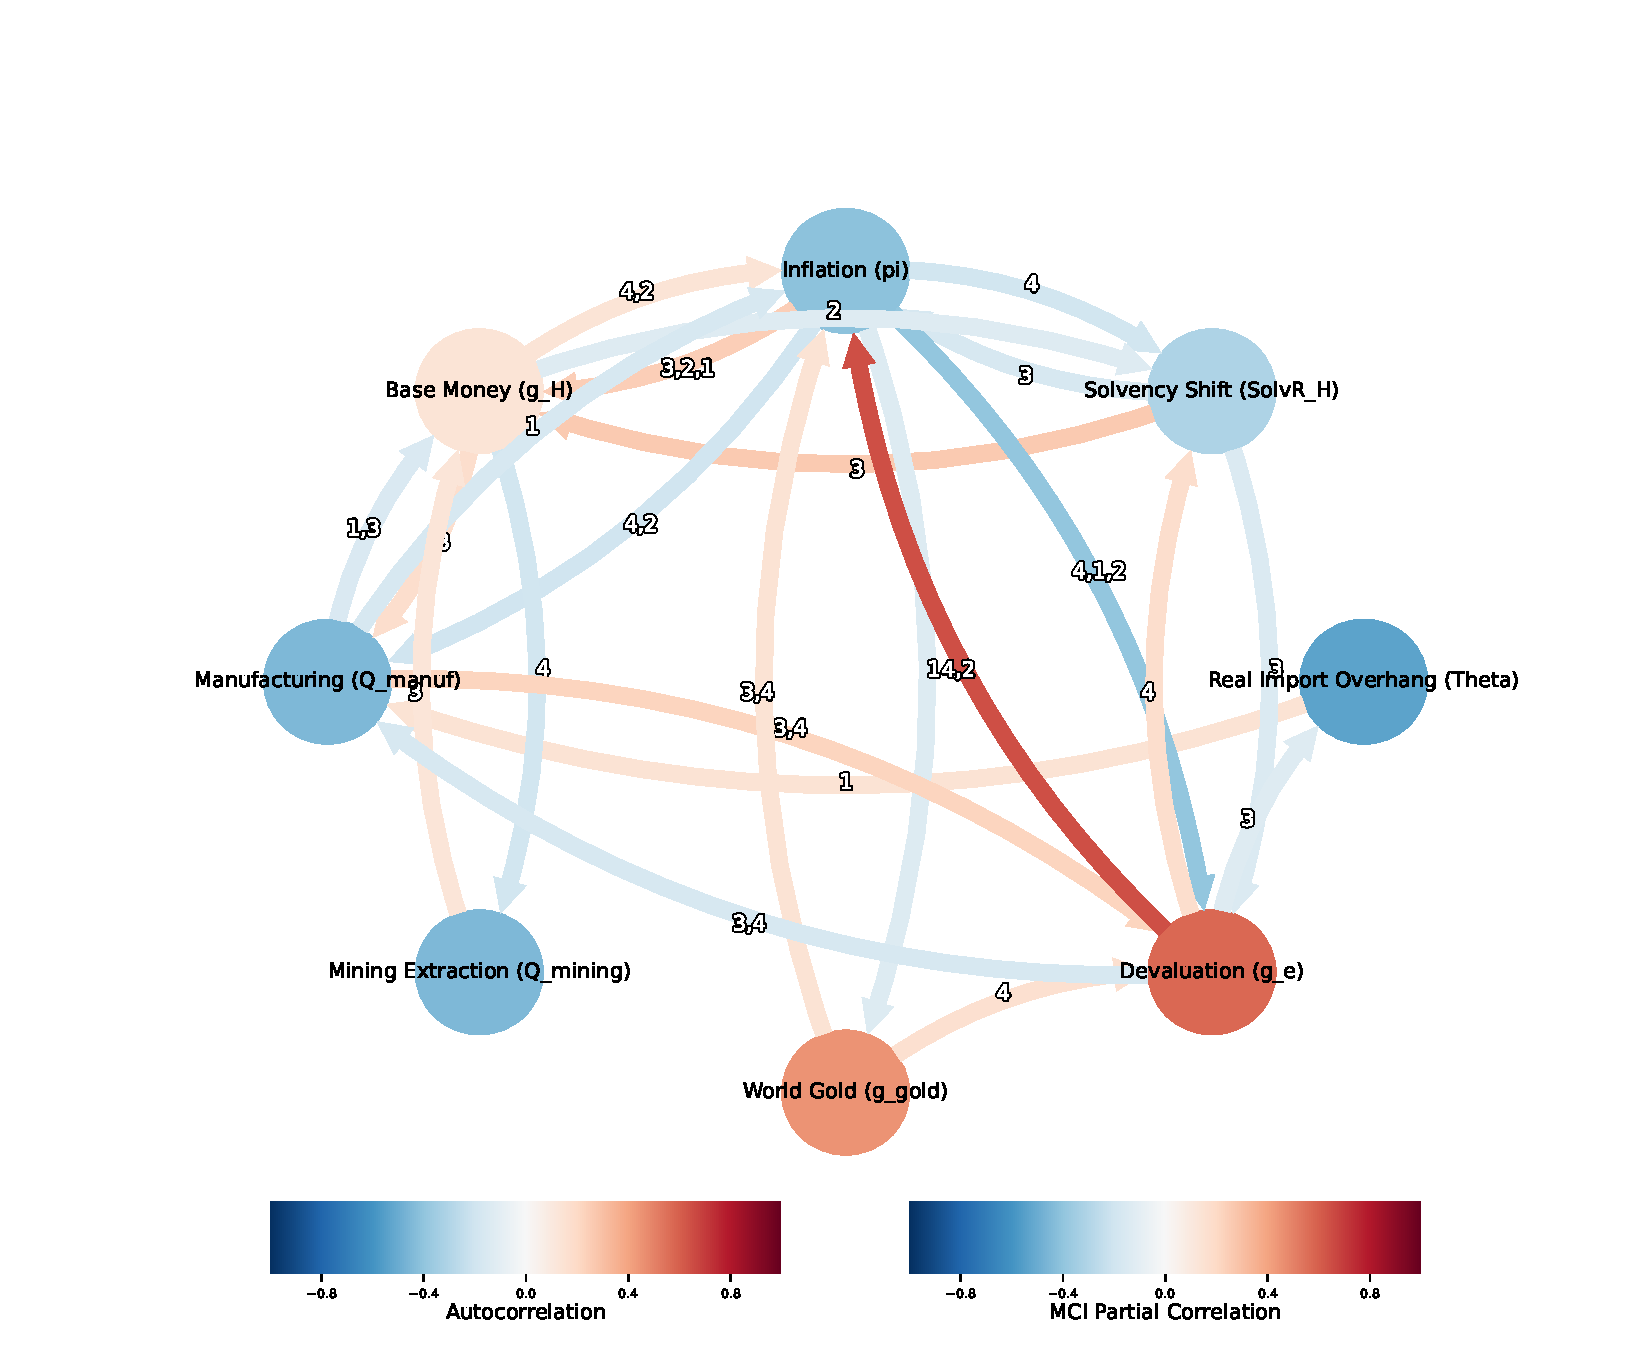
\includegraphics[width=0.84\textwidth]{figures/dag_pcmci_monthly_gate.pdf}
\vspace{1.0em}
\begin{minipage}{0.96\textwidth}
\footnotesize \textit{Notes:} Algorithmic circular time-series causal discovery network estimated using Tigramite PCMCI \citep{Runge2019} on the 8-variable monthly macroeconomic system ($N=250$, 1960:01--1980:12) with partial correlation conditional independence tests ($\alpha = 0.05$, FDR-corrected). Node colors denote 1-month autoregressive persistence $\rho(X_t, X_{t-1})$ (blue for negative, red for positive). Directed curved edges represent lag-specific Momentary Conditional Independence (MCI) partial correlations surviving conditioning on the minimal parent sets of both the driver and the target ($\widehat{\mathcal{P}}(X^j_t)$ and $\widehat{\mathcal{P}}(X^i_{t-\tau})$). Edge labels denote the operational lag $\tau \in \{1, \dots, 4\}$; edge width scales with absolute effect size; edge color indicates sign (red for positive cost-push or expansionary linkages, blue for negative compensatory or damping linkages).
\end{minipage}
\end{figure}

\clearpage

\begin{table}[htbp]
\centering
\small
\caption{Full-System PCMCI Momentary Conditional Independence (MCI) Directed Link Tests (1960--1980)}
\label{tab:pcmci_monthly_gate}
\label{tab:pcmci_mci_links}
\begin{tabularx}{\textwidth}{>{\RaggedRight}p{4.5cm}cc>{\RaggedRight}p{2.0cm}>{\RaggedRight}X}
\toprule
\textbf{Directed Link Tested} & \textbf{Lag ($\tau$)} & \textbf{MCI Partial Corr.} & \textbf{$p$-value} & \textbf{Causal Status (FDR $q < 0.05$)} \\
\midrule
$\pi_{t-3} \to g_{H,t}$ (Reverse Accomm.) & $\tau = 3$ & +0.247 & $0.0001$*** & Retained directed edge ($\pi \to g_H$) \\
$g_{H,t-\tau} \to \pi_t$ (Forward Monetarist) & $\tau = 4$ & +0.138 & $0.0350$** & Excluded (FDR $q > 0.10$, zero direct link) \\
$\Delta \ln \text{SolvR}^H_{t-3} \to g_{H,t}$ (Defensive Emission) & $\tau = 3$ & +0.264 & $< 0.0001$*** & Retained directed edge ($\text{SolvR}^H \to g_H$) \\
$\Delta \ln \text{SolvR}^H_{t-3} \to \pi_t$ (Solvency Gate) & $\tau = 3$ & -0.165 & $0.0115$** & Retained directed edge ($\text{SolvR}^H \to \pi$) \\
$g_{e, t-4} \to \pi_t$ (External Pass-Through) & $\tau = 4$ & +0.644 & $< 0.0001$*** & Retained directed edge ($g_e \to \pi$) \\
$\pi_{t-4} \to g_{e, t}$ (Forced Devaluation) & $\tau = 4$ & -0.396 & $< 0.0001$*** & Retained directed edge ($\pi \to g_e$) \\
$\Delta \ln \Theta_{t-1} \to g_{\text{Manuf}, t}$ (Import Constraint) & $\tau = 1$ & +0.142 & $0.0287$** & Retained directed edge ($\Theta \to \text{Manuf}$) \\
$g_{H, t-3} \to g_{\text{Manuf}, t}$ (Idle Reactivation) & $\tau = 3$ & +0.177 & $0.0064$*** & Retained directed edge ($g_H \to \text{Manuf}$) \\
$g_{\text{Manuf}, t-1} \to \pi_t$ (Price Suppression) & $\tau = 1$ & -0.168 & $0.0101$** & Retained directed edge ($\text{Manuf} \to \pi$) \\
$g_{H, t-4} \to g_{\text{Mining}, t}$ (Enclave Decoupling) & $\tau = 4$ & -0.189 & $0.0035$*** & Retained directed edge ($g_H \to \text{Mining}$) \\
$g_{P,\text{gold}, t-4} \to g_{e, t}$ (Gold Cost Push) & $\tau = 4$ & +0.163 & $0.0119$** & Retained directed edge ($P^{\text{gold}} \to g_e$) \\
$g_{P,\text{gold}, t-3} \to \pi_t$ (Gold Inflation) & $\tau = 3$ & +0.146 & $0.0241$** & Retained directed edge ($P^{\text{gold}} \to \pi$) \\
$\pi_{t-\tau} \to \Delta \ln \Theta_t$ (Exogeneity Check) & $\tau \in [1,4]$ & -0.074 & $0.2545$ & Block-exogenous ($p = 0.255$) \\
$g_{H,t-\tau} \to g_{P,\text{gold}, t}$ (Exogeneity Check) & $\tau \in [1,4]$ & -0.107 & $0.1004$ & Block-exogenous ($p = 0.100$) \\
$g_{H,t-\tau} \to \Delta \ln \text{SolvR}^H_t$ (Monetary Drain) & $\tau \in [1,4]$ & -0.131 & $0.0449$** & Excluded (zero direct link) \\
\bottomrule
\end{tabularx}
\begin{minipage}{\textwidth}
\vspace{0.3em}
\footnotesize \textit{Notes:} Monthly series spanning 1960:01--1980:12 ($N=250$). Estimated using Tigramite PCMCI \citep{Runge2019} on the 8-variable system with partial correlation conditional independence tests evaluated across lags $\tau \in \{1, \dots, 4\}$. Minimal conditioning parent sets $\widehat{\mathcal{P}}(X^j_t)$ and $\widehat{\mathcal{P}}(X^i_{t-\tau})$ are selected in the PC$_1$ phase. False discovery rates are controlled via the Benjamini--Hochberg procedure at FDR $q < 0.05$. Significance: $^{***} p < 0.01$, $^{**} p < 0.05$, $^{*} p < 0.10$. Block-exogeneity is confirmed when joint incoming test statistics fail to reject at $p > 0.10$.
\end{minipage}
\end{table}
